\documentclass{article}
\usepackage[utf8]{inputenc}
\setlength{\parskip}{5pt} % esp. entre parrafos
\setlength{\parindent}{0pt} % esp. al inicio de un parrafo
\usepackage{listings} % listings
\usepackage{color} %colores
\usepackage{amsmath} % mates
\usepackage[sort&compress,numbers]{natbib} % referencias
\usepackage{url} % que las URLs se vean lindos
\usepackage[top=15mm,left=20mm,right=20mm,bottom=25mm]{geometry} % margenes
\usepackage{hyperref} % ligas de URLs
\usepackage{graphicx} % poner figuras
\usepackage[spanish,es-tabla]{babel} % nombre tablas
\usepackage{caption}
\usepackage{subcaption}



\definecolor{mypink}{rgb}{0.976, 0.462, 0.847}
\definecolor{mygray}{rgb}{0.976, 0.980, 0.980}
\definecolor{myblue}{rgb}{0.258, 0.682, 1}
\definecolor{mypink2}{rgb}{0.525, 0.054, 0.4}
\lstset{ 
  backgroundcolor=\color{mygray},
  commentstyle=\color{myblue},
  keywordstyle=\color{mypink}, 
  numberstyle=\tiny\color{mypink}
  stringstyle=\color{mypink2}, 
  breaklines=true,
}

\title{Tarea 9}
\author{Eduardo Navarro}
\date{Octubre 2021}

\begin{document}

\maketitle

\section{Introducción}
En esta práctica se analizaron las interacciones de las fuerzas atractoras debido a la gravedad causada por la masa y la atracción y repulsión por la carga.

\section{Desarrollo}
Con las instrucciones de la tarea \cite{particulas} y lo visto en clase \cite{twitchsimu} se le hicieron modificaciones al código para obtener la fuerza dependiente de la masa y la carga \cite{maria}. así mismo se añadió un \texttt{for} para hacer las repeticiones y el correspondiente análisis estadístico.

\begin{lstlisting} [language=R, caption= Código para la obtención de las fuerzas.]
for (repe in repeticiones) {
p <- data.frame(repe, x = rnorm(n), y=rnorm(n), c=rnorm(n), m=rnorm(n))
...
p$c <-  2 * (p$c - cmin) / (cmax - cmin) - 1 # cargas son entre -1 y 1 # cargas son entre -1 y 1
p$g <- round(5 * p$c) # coloreamos segun la carga a 11 niveles de -5 a 5
mmax=max(p$m)
mmin=min(p$m)
p$m=(p$m - mmin) / (mmax - mmin) + 0.01
...
fuerza <- function(i) {
 xi <- p[i,]$x
 yi <- p[i,]$y
 ci <- p[i,]$c
 mi <- p[i,]$m 
 fx <- 0
...
  fy <- fy - dy * factor
  }
  return(c(fx, fy)/(mi)) 
}
\end{lstlisting}
Se añadió también la velocidad \cite{maria}.

\begin{lstlisting} [language=R, caption= Código para la obtención de la velocidad.]

p$vel=numeric(n)
for (iter in 1:tmax) {
 f <- foreach(i = 1:n, .combine=c) %dopar% fuerza(i)
 delta <- 0.02 / max(abs(f)) # que nadie desplace una paso muy largo
 p$x <- foreach(i = 1:n, .combine=c) %dopar% max(min(p[i,]$x + delta * f[c(TRUE, FALSE)][i], 1), 0)
 p$y <- foreach(i = 1:n, .combine=c) %dopar% max(min(p[i,]$y + delta * f[c(FALSE, TRUE)][i], 1), 0)
 v <- foreach(i=1:n,.combine=c)%dopar% sqrt((delta * f[c(TRUE, FALSE)][i])^2 + (delta * f[c(FALSE, TRUE)][i])^2)
 p$vel=p$vel+v
\end{lstlisting}

 Con esto se generaron los datos de la tabla \ref{tabla1} y se procedió a graficar \ref{grafica1}, \ref{grafica2}.
 
 \begin{table}[h!]
\centering
\caption{Ejemplo de datos obtenidos.}
\label{tabla1}
\begin{tabular}{|c|r|r|r|r|r|r|}
\hline
\textbf{Repetición} & \multicolumn{1}{c|}{\textbf{x}} & \multicolumn{1}{c|}{\textbf{y}} & \multicolumn{1}{c|}{\textbf{c}} & \multicolumn{1}{c|}{\textbf{m}} & \multicolumn{1}{c|}{\textbf{g}} & \multicolumn{1}{c|}{\textbf{vel}} \\ \hline
1 & 0.485705 & 0.42889 & 0.297992 & 0.151728 & 1 & 0.060159 \\ \hline
1 & 0.213222 & 0.436536 & -0.21141 & 0.458048 & -1 & 0.012109 \\ \hline
1 & 0.89874 & 0.680653 & 0.038923 & 0.81409 & 0 & 0.026078 \\ \hline
1 & 0.588958 & 0.673364 & -0.23507 & 0.433041 & -1 & 0.00786 \\ \hline
1 & 0.463067 & 0.282932 & -0.38233 & 0.165334 & -2 & 0.030852 \\ \hline
1 & 0.266291 & 0.741391 & -0.76117 & 0.252549 & -4 & 0.02669 \\ \hline
1 & 0.763601 & 0.322711 & -0.7211 & 0.341185 & -4 & 0.009858 \\ \hline
\end{tabular}
\end{table}

\begin{figure} [h!]% figura
\renewcommand{\figurename}{Gráfica}
    \centering
    \caption{ Velocidad a masa y carga dadas.}
    \label{grafica1}
    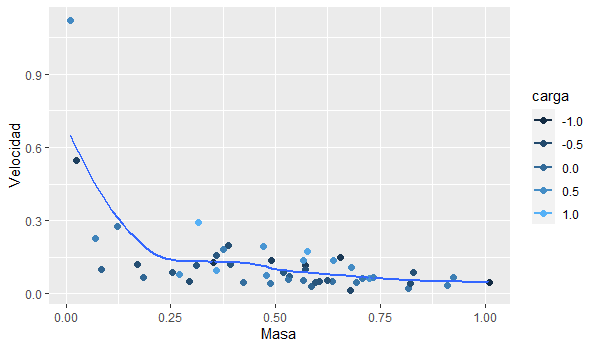
\includegraphics[width=150mm]{grafica1.png} % archivo
\end{figure}
\newpage

\begin{figure} [h!]% figura
\renewcommand{\figurename}{Gráfica}
    \centering
    \caption{ Velocidad a carga y masa dadas.}
    \label{grafica2}
    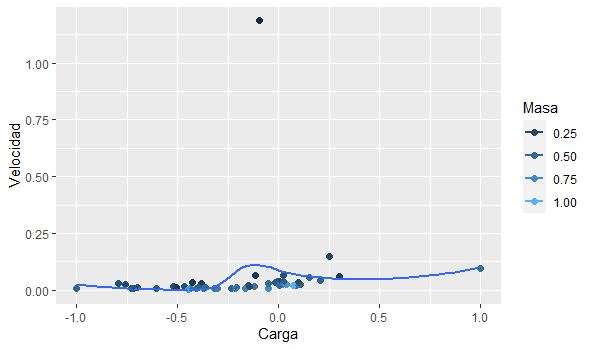
\includegraphics[width=150mm]{grafica2.png} % archivo
\end{figure}

\begin{lstlisting} [language=R, caption= Código para la obtención de las gráficas.]
#carga contra velocidad
ggplot(data = p, aes(x= c, y= vel, color= m))+
  geom_point(size=2)+
  geom_smooth(method = "loess", se=FALSE, formula =y ~ x)+
  stat_summary(fun = mean, geom = "point",
               size = 0.7, fill = "black")+
  guides(scale = "none", color=guide_legend(title = "Masa"))+
  scale_x_continuous(name = "Carga")+
  scale_y_continuous(name = "Velocidad")+
  theme(plot.title = element_text(hjust = 0.5))

#masa contra velocidad
ggplot(data = p, aes(x= m, y= vel, color= c))+
  geom_point(size=2)+
  geom_smooth(method = "loess", se=FALSE, formula =y ~ x)+
  stat_summary(fun = mean, geom = "point",
               size = 0.7, fill = "black")+
  guides(scale = "none", color=guide_legend(title = "carga"))+
  scale_x_continuous(name = "Masa")+
  scale_y_continuous(name = "Velocidad")+
  theme(plot.title = element_text(hjust = 0.5))
\end{lstlisting}

Después se fijó la masa para ver las velocidades obtenidas cambiando el código.

\begin{lstlisting} [language=R, caption= Código para las masas fijas.]
library(ggplot2)
    
n <- 20

datos<- data.frame()

mass<-seq(0.1,0.9,0.2)

repeticiones<- 1:10
for (masas in mass) {

for (repe in repeticiones) {
p <- data.frame(repe, x = rnorm(n), y=rnorm(n), c=rnorm(n), m=rnorm(n))
...
p$c <- 2 * (p$c - cmin) / (cmax - cmin) - 1 # cargas son entre -1 y 1
p$g <- round(5 * p$c) # coloreamos segun la carga a 11 niveles de -5 a 5
mmax=max(p$m)
mmin=min(p$m)
p$m=masas
\end{lstlisting}

Con esto se procedió a generar la gráfica \ref{grafica3} y su correspondiente análisis.

\begin{figure} [h!]% figura
\renewcommand{\figurename}{Gráfica}
    \centering
    \caption{ Velocidad con masa fija.}
    \label{grafica3}
    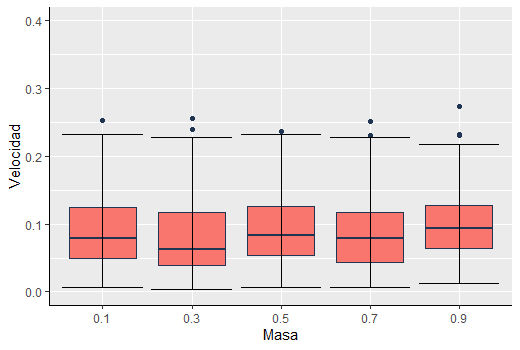
\includegraphics[width=150mm]{grafica3.png} % archivo
\end{figure}

\begin{lstlisting} [language=R, caption= Código para la gráfica de masas fijas y análisis estadístico.]
datos$m = as.factor(datos$m)

ggplot(datos, aes(x=m , y=vel , fill= repe)) + # fill=name allow to automatically dedicate a color for each group
  geom_boxplot(fill = "#F8766D", colour = "#1F3552")+
  stat_boxplot(geom = "errorbar", width = 0.9)+
  theme(axis.line = element_line(colour = "black", size = 0.25))+
  coord_cartesian(ylim = c(0,0.4))+
  labs(x="Masa", y= "Velocidad")
  
library(tidyverse)

resulmasa<-datos%>%
  group_by(m) %>%
  summarise(
    
    promedio = mean(vel, na.rm = TRUE),
    desviacion_std = sd(vel, na.rm = TRUE),
    varianza = sd(vel, na.rm = TRUE)^2,
    mediana = median(vel, na.rm = TRUE),
    rango_intercuartil = IQR(vel, na.rm = TRUE)
  )

mshapiro<-tapply(datos$vel, datos$m, shapiro.test)

kruskal.test(vel~m, data=datos)

mwilcox<-pairwise.wilcox.test(datos$vel, datos$m)
\end{lstlisting}

De la gráfica \ref{grafica3} podemos ver que a masa constante la velocidad depende solo de la carga por lo que no se aprecia un cambio. Se realizaron pruebas de  Shapiro–Wilk \cite{shapiro} y Kruskal-Wallis \cite{Kruskall} junto con la prueba Wilcox \cite{pairwise} para el análisis de datos.

\begin{table}[h!]
\centering
\caption{Datos estadísticos obtenidos para la masa fija.}
\label{tabla2}
\begin{tabular}{|c|r|r|r|r|r|r|}
\hline
\textbf{m} & \multicolumn{1}{c|}{\textbf{Promedio}} & \multicolumn{1}{c|}{\textbf{Desviación std}} & \multicolumn{1}{c|}{\textbf{Varianza}} & \multicolumn{1}{c|}{\textbf{Mediana}} & \multicolumn{1}{c|}{\textbf{Rango intercuartil}} \\ \hline
0.1 & 0.092401742 & 0.056848948 & 0.003231803 & 0.078188318 & 0.074729255  \\ \hline
0.3 & 0.081543654 & 0.056451991 & 0.003186827 & 0.062769848 & 0.078253016 \\ \hline
0.5 & 0.093686684 & 0.052818425 & 0.002789786 & 0.083157794 & 0.072763081  \\ \hline
0.7 & 0.087835523 & 0.05601731 & 0.003137939 & 0.078490882 & 0.073722512  \\ \hline
0.9 & 0.101696009 & 0.049671587 & 0.002467267 & 0.094239537 & 0.06306384  \\ \hline
\end{tabular}
\end{table}

\begin{table}[h!]
\centering
\caption{Resultados de la prueba Shapiro–Wilk para la masa fija.}
\label{tabla3}
\begin{tabular}{|c|r|r|}
\hline
\textbf{m} & \multicolumn{1}{c|}{\textbf{W}} & \multicolumn{1}{c|}{\textbf{P}} \\ \hline
0.1 & 0.92571 & $1.56\times 10^{-8}$ \\ \hline
0.3 & 0.90285 & $3.83\times 10^{-10}$ \\ \hline
0.5 & 0.95083 & $2.27\times 10^{-6}$ \\ \hline
0.7 & 0.92354 & $1.07\times 10^{-8}$ \\ \hline
0.9 & 0.96021 & $2.08\times 10^{-5}$ \\ \hline
\end{tabular}
\end{table}

\begin{table}[h!]
\centering
\caption{Resultados de la prueba Kruskal-Wallis para la masa fija.}
\label{tabla4}
\begin{tabular}{|l|l|}
\hline
\multicolumn{1}{|c|}{\textbf{H(4)}} & \multicolumn{1}{c|}{\textbf{P}} \\ \hline
25.141 & $4.71\times 10^{-5}$ \\ \hline
\end{tabular}
\end{table}


\begin{table}[h!]
\centering
\caption{Resultados de la prueba por parejas de Wilcox para la masa fija.}
\label{tabla5}
\begin{tabular}{|c|r|r|c|c|}
\hline
m & \multicolumn{1}{c|}{0.1} & \multicolumn{1}{c|}{0.3} & 0.5 & 0.7 \\ \hline
0.3 & 0.116 & \multicolumn{1}{c|}{-} & - & - \\ \hline
0.5 & 0.871 & 0.027 & - & - \\ \hline
0.7 & 0.871 & 0.56 & \multicolumn{1}{r|}{0.56} & - \\ \hline
0.9 & 0.092 & $1.8\times 10^{-5}$ & \multicolumn{1}{r|}{0.327} & \multicolumn{1}{r|}{0.008} \\ \hline
\end{tabular}
\end{table}

Se volvió a cambiar el código para solo tomar en cuenta las repeticiones y medir la velocidad en relación a la carga con g que toma números enteros obteniendo así la grafica \ref{grafica4}.

\begin{lstlisting} [language=R, caption= Código para la relación con la carga y masa.]
library(ggplot2)
    
n <- 50

datos<- data.frame()

repeticiones<- 1:15
  
for (repe in repeticiones) {
p <- data.frame(repe, x = rnorm(n), y=rnorm(n), c=rnorm(n), m=rnorm(n))
...
cmax <- max(p$c)
cmin <- min(p$c)
p$c <-  2 * (p$c - cmin) / (cmax - cmin) - 1 # cargas son entre -1 y 1 # cargas son entre -1 y 1
p$g <- round(5 * p$c) # coloreamos segun la carga a 11 niveles de -5 a 5
mmax=max(p$m)
mmin=min(p$m)
p$m=(p$m - mmin) / (mmax - mmin) + 0.01
\end{lstlisting}

\begin{figure} [h!]% figura
\renewcommand{\figurename}{Gráfica}
    \centering
    \caption{ Velocidad tomando en cuenta la carga y masa.}
    \label{grafica4}
    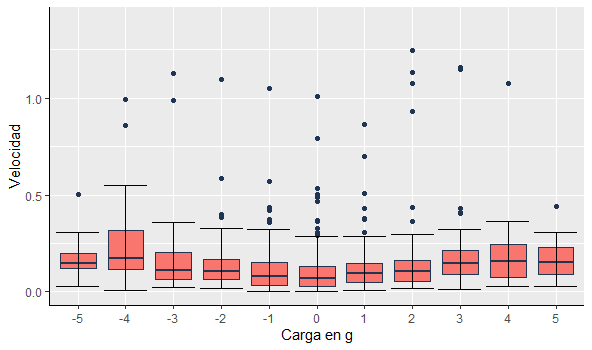
\includegraphics[width=150mm]{grafica4.png} % archivo
\end{figure}

\begin{lstlisting}[language=R, caption= Código para la gráfica y pruebas estadísticas tomando en cuenta la velocidad con la carga y masa.]

datos$g = as.factor(datos$g)

ggplot(datos, aes(x=g , y=vel , fill= repe)) + # fill=name allow to automatically dedicate a color for each group
  geom_boxplot(fill = "#F8766D", colour = "#1F3552")+
  stat_boxplot(geom = "errorbar", width = 0.9)+
  theme(axis.line = element_line(colour = "black", size = 0.25))+
  coord_cartesian(ylim = c(0,1.4))+
  labs(x="Carga en g", y= "Velocidad")

library(tidyverse)

resulcarg<-datos%>%
  group_by(g) %>%
  summarise(
    
    promedio = mean(vel, na.rm = TRUE),
    desviacion_std = sd(vel, na.rm = TRUE),
    varianza = sd(vel, na.rm = TRUE)^2,
    mediana = median(vel, na.rm = TRUE),
    rango_intercuartil = IQR(vel, na.rm = TRUE)
  )

cshapiro<-tapply(datos$vel, datos$g, shapiro.test)

kruskal.test(vel~g, data=datos)

cwilcox<-pairwise.wilcox.test(datos$vel, datos$g)
\end{lstlisting}

De la gráfica \ref{grafica4} podemos observar puntos máximos en la velocidad independientes de la carga. Estos son correspondientes a los datos de la tabla \ref{tabla6}. 

\begin{table}[h!]
\centering
\caption{Ejemplo de datos obtenidos de la velocidad con la carga y masa.}
\label{tabla6}
\begin{tabular}{|c|r|r|r|r|r|r|}
\hline
\textbf{Repetición} & \multicolumn{1}{c|}{\textbf{x}} & \multicolumn{1}{c|}{\textbf{y}} & \multicolumn{1}{c|}{\textbf{c}} & \multicolumn{1}{c|}{\textbf{m}} & \multicolumn{1}{c|}{\textbf{g}} & \multicolumn{1}{c|}{\textbf{vel}} \\ \hline
13 & 0.594651 & 0.544753 & 0.45104 & 0.01 & 2 & 1.248722 \\ \hline
3 & 0.587369 & 0.495097 & 0.696364 & 0.01 & 3 & 1.156986 \\ \hline
6 & 0.489923 & 0.559607 & 0.555117 & 0.01 & 3 & 1.146562 \\ \hline
7 & 0.539666 & 0.499276 & 0.408238 & 0.01 & 2 & 1.133769 \\ \hline
5 & 0.454857 & 0.453346 & -0.56575 & 0.01 & -3 & 1.129291 \\ \hline
9 & 0.392561 & 0.444595 & -0.39887 & 0.01 & -2 & 1.099558 \\ \hline
8 & 0.510297 & 0.531619 & 0.826534 & 0.01 & 4 & 1.077581 \\ \hline
\end{tabular}
\end{table}

\begin{table}[h!]
\centering
\caption{Datos estadísticos obtenidos para la velocidad con la carga y masa.}
\label{tabla7}
\begin{tabular}{|c|r|r|r|r|r|}
\hline
\textbf{g} & \multicolumn{1}{c|}{\textbf{Promedio}} & \multicolumn{1}{c|}{\textbf{Desviacion std}} & \multicolumn{1}{c|}{\textbf{Varianza}} & \multicolumn{1}{c|}{\textbf{Mediana}} & \multicolumn{1}{c|}{\textbf{Rango intercuartil}} \\ \hline
-5 & 0.167014 & 0.095310357 & 0.009084064 & 0.149072061 & 0.075028234 \\ \hline
-4 & 0.236642 & 0.209683653 & 0.043967234 & 0.170961659 & 0.202454132 \\ \hline
-3 & 0.167241 & 0.187540665 & 0.035171501 & 0.112627254 & 0.138985248 \\ \hline
-2 & 0.144425 & 0.145459065 & 0.02115834 & 0.106956546 & 0.106341214 \\ \hline
-1 & 0.112811 & 0.132099698 & 0.01745033 & 0.079946386 & 0.122759194 \\ \hline
0 & 0.114287 & 0.14658308 & 0.021486599 & 0.067285049 & 0.10393401 \\ \hline
1 & 0.127883 & 0.135504027 & 0.018361341 & 0.094959264 & 0.099753735 \\ \hline
2 & 0.169288 & 0.236013627 & 0.055702432 & 0.107620206 & 0.108982644 \\ \hline
3 & 0.195482 & 0.20685509 & 0.042789028 & 0.145127425 & 0.122490707 \\ \hline
4 & 0.186557 & 0.182861296 & 0.033438254 & 0.157073824 & 0.166537393 \\ \hline
5 & 0.170218 & 0.101373483 & 0.010276583 & 0.153077881 & 0.137837886 \\ \hline
\end{tabular}
\end{table}

\newpage

\begin{table}[h!]
\centering
\caption{Resultados de la prueba Shapiro–Wilk para la velocidad con la carga y masa.}
\label{tabla8}
\begin{tabular}{|c|r|r|}
\hline
\textbf{g} & \multicolumn{1}{c|}{\textbf{W}} & \multicolumn{1}{c|}{\textbf{P}} \\ \hline
-5 & 0.86324, & 0.002598 \\ \hline
-4 & 0.78386, & $6.27\times 10^{-6}$ \\ \hline
-3 & 0.6118, & $1.23\times 10^{-11}$ \\ \hline
-2 & 0.66017, & $1.00\times 10^{-12}$ \\ \hline
-1 & 0.67341, & $3.59\times 10^{-15}$ \\ \hline
0 & 0.65585, & $5.75\times 10^{-16}$ \\ \hline
1 & 0.71089, & $1.35\times 10^{-12}$ \\ \hline
2 & 0.52643, & $2.86\times 10^{-14}$ \\ \hline
3 & 0.59384, & $2.07\times 10^{-11}$ \\ \hline
4 & 0.63461, & $5.62\times 10^{-8}$ \\ \hline
5 & 0.9316, & 0.1482 \\ \hline
\end{tabular}
\end{table}

\begin{table}[h!]
\centering
\caption{Resultados de la prueba Kruskal-Wallis para la velocidad con la carga y masa.}
\label{tabla9}
\begin{tabular}{|c|c|}
\hline
H(10) & P \\ \hline
\multicolumn{1}{|r|}{74.575} & \multicolumn{1}{r|}{$5.76\times 10^{-12}$} \\ \hline
\end{tabular}
\end{table}

\begin{table}[h!]
\centering
\caption{Resultados de la prueba por parejas de Wilcox para la velocidad con la carga y masa.}
\label{tabla10}
\begin{tabular}{|c|r|r|r|r|r|c|c|c|c|c|}
\hline
g & \multicolumn{1}{c|}{-5} & \multicolumn{1}{c|}{-4} & \multicolumn{1}{c|}{-3} & \multicolumn{1}{c|}{-2} & \multicolumn{1}{c|}{-1} & 0 & 1 & 2 & 3 & 4 \\ \hline
-4 & 1 & \multicolumn{1}{c|}{-} & \multicolumn{1}{c|}{-} & \multicolumn{1}{c|}{-} & \multicolumn{1}{c|}{-} & - & - & - & - & - \\ \hline
-3 & 1 & 0.50314 & \multicolumn{1}{c|}{-} & \multicolumn{1}{c|}{-} & \multicolumn{1}{c|}{-} & - & - & - & - & - \\ \hline
-2 & 1 & 0.07077 & 1 & \multicolumn{1}{c|}{-} & \multicolumn{1}{c|}{-} & - & - & - & - & - \\ \hline
-1 & 0.01979 & 0.00034 & 0.06633 & 0.17082 & \multicolumn{1}{c|}{-} & - & - & - & - & - \\ \hline
0 & 0.00452 & 0.00012 & 0.01979 & 0.03703 & 1 & - & - & - & - & - \\ \hline
1 & 0.08363 & 0.00452 & 1 & 1 & 1 & \multicolumn{1}{r|}{1} & - & - & - & - \\ \hline
2 & 0.48793 & 0.07535 & 1 & 1 & 0.33313 & \multicolumn{1}{r|}{0.06633} & \multicolumn{1}{r|}{1} & - & - & - \\ \hline
3 & 1 & 1 & 1 & 0.60812 & 0.00047 & \multicolumn{1}{r|}{$6.4\times 10^{-5}$} & \multicolumn{1}{r|}{0.02534} & \multicolumn{1}{r|}{0.35531} & - & - \\ \hline
4 & 1 & 1 & 1 & 1 & 0.02167 & \multicolumn{1}{r|}{0.00561} & \multicolumn{1}{r|}{0.24028} & \multicolumn{1}{r|}{1} & \multicolumn{1}{r|}{1} & - \\ \hline
5 & 1 & 1 & 1 & 1 & 0.06633 & \multicolumn{1}{r|}{0.0313} & \multicolumn{1}{r|}{0.33686} & \multicolumn{1}{r|}{1} & \multicolumn{1}{r|}{1} & \multicolumn{1}{r|}{1} \\ \hline
\end{tabular}
\end{table}
Se obtuvieron varias imágenes donde se aprecia el movimiento de las partículas a cierta velocidad con sus respectivas cargas y masas.

\begin{lstlisting} [language=R, caption= Código para la obtención de las imágenes.]
#Estado inicial
png(paste("t9_t", 0, tl, ".png", sep=""),width = 800,height = 700)
print( ggplot(data=p, aes(x=x ,y=y, size=m, col=colores[p$g+6]) )
       +geom_point(show.legend =  TRUE)+xlim(c(0,1))+ylim(c(0,1))+  
         ggtitle(paste("Estado inicial"))
       + scale_shape_discrete(name  ="Carga")+ 
         scale_colour_discrete(name  ="Carga", labels=seq(-5,5)))
graphics.off()
...
 tl <- paste(iter, "", sep="")
 while (nchar(tl) < digitos) {
    tl <- paste("0", tl, sep="")
  }
 png(paste("t9_t", 0, tl, ".png", sep=""),width = 800,height = 700)
 print( ggplot(data=p, aes(x=x ,y=y, size=m, col=colores[p$g+6]) )
        +geom_point(show.legend =  TRUE)+xlim(c(0,1))+ylim(c(0,1))+  
        scale_shape_discrete(name  ="Carga")+ 
        ggtitle(paste(tl))+
        scale_colour_discrete(name  ="Carga", labels=seq(-5,5)))
 graphics.off()
 
\end{lstlisting}


\begin{figure}[h!]
\centering
\caption{Movimiento de las partículas en relación a su velocidad, carga y masa.}
\begin{subfigure}[b]{0.3\linewidth}
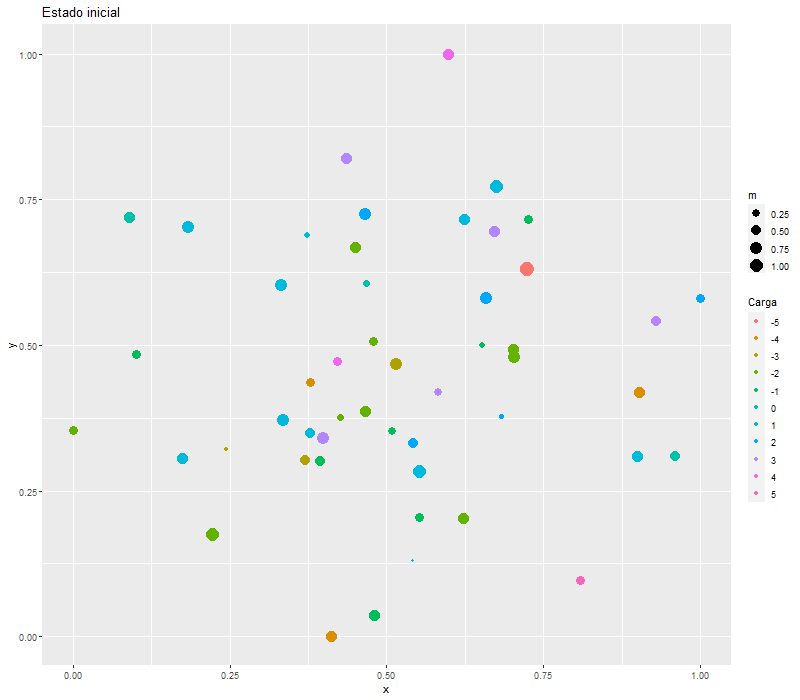
\includegraphics[width=\linewidth]{grafica5.png}
\caption{Paso 1.}
\label{a}
\end{subfigure}
\begin{subfigure}[b]{0.3\linewidth}
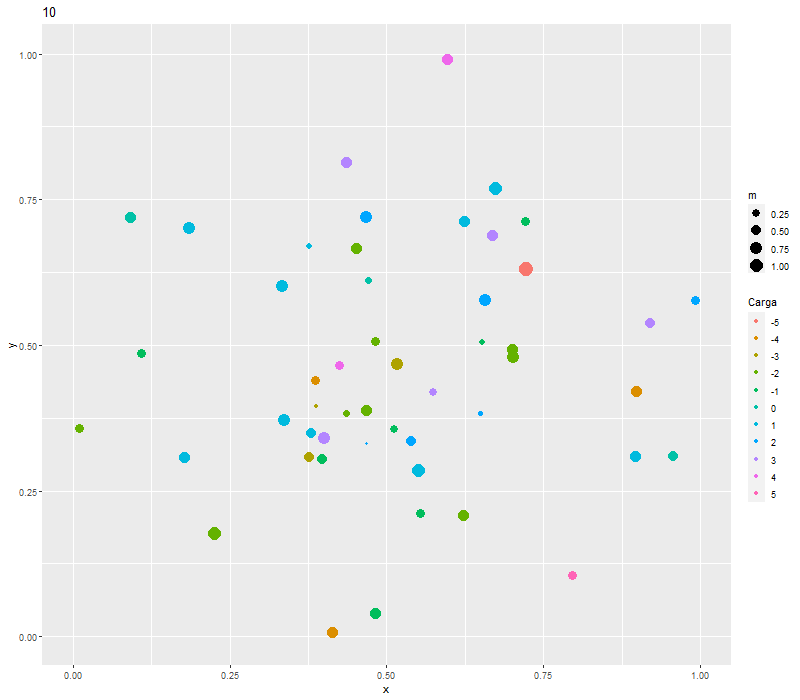
\includegraphics[width=\linewidth]{grafica6.png}
\caption{Paso 10.}
\label{b}
\end{subfigure}
\begin{subfigure}[b]{0.3\linewidth}
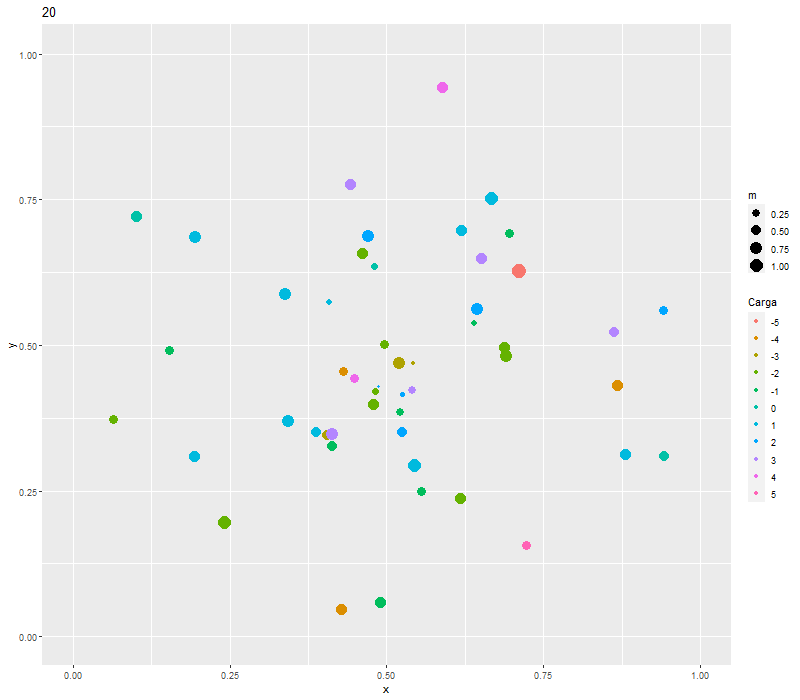
\includegraphics[width=\linewidth]{grafica7.png}
\caption{Paso 20.}
\label{c}
\end{subfigure}
\begin{subfigure}[b]{0.3\linewidth}
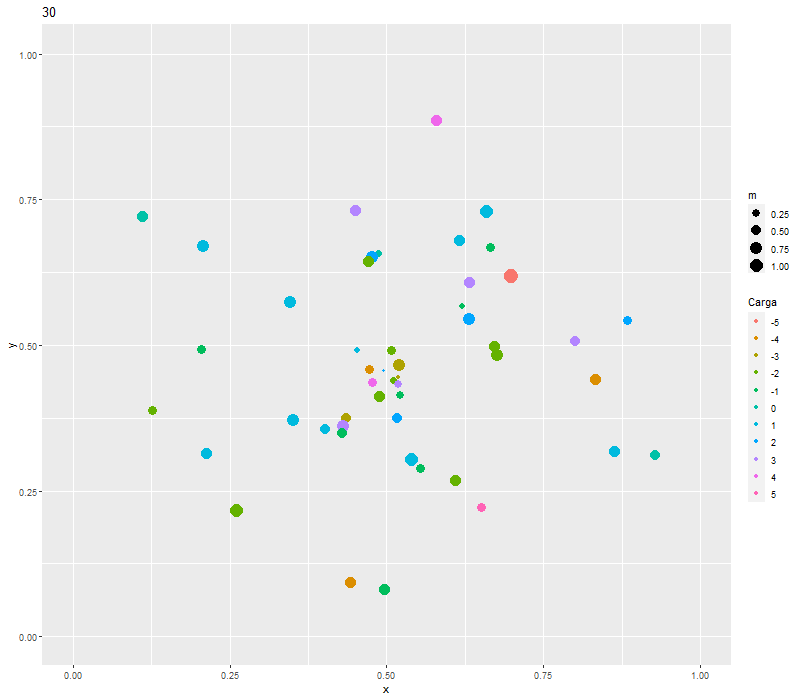
\includegraphics[width=\linewidth]{grafica8.png}
\caption{Paso 30.}
\label{d}
\end{subfigure}
\begin{subfigure}[b]{0.3\linewidth}
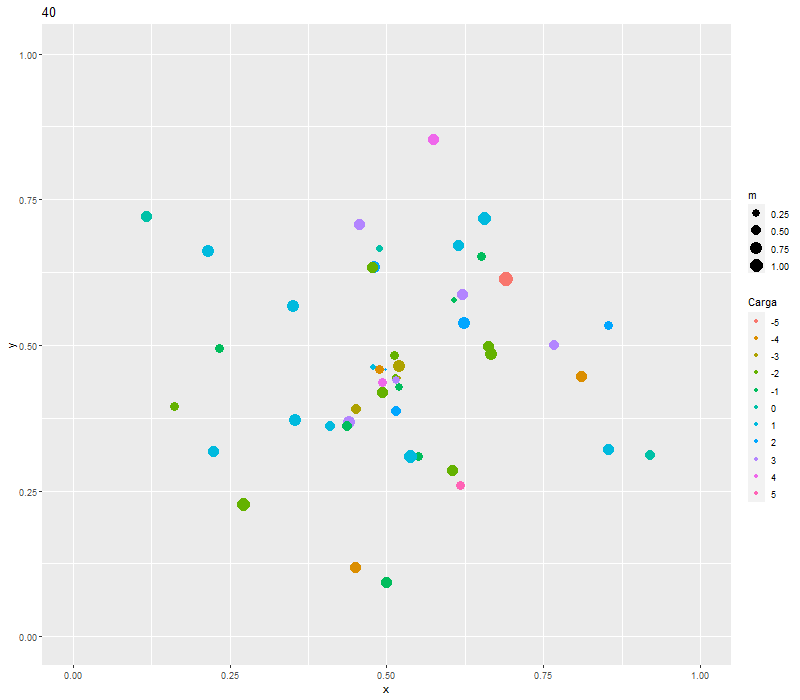
\includegraphics[width=\linewidth]{grafica9.png}
\caption{Paso 40.}
\label{e}
\end{subfigure}
\begin{subfigure}[b]{0.3\linewidth}
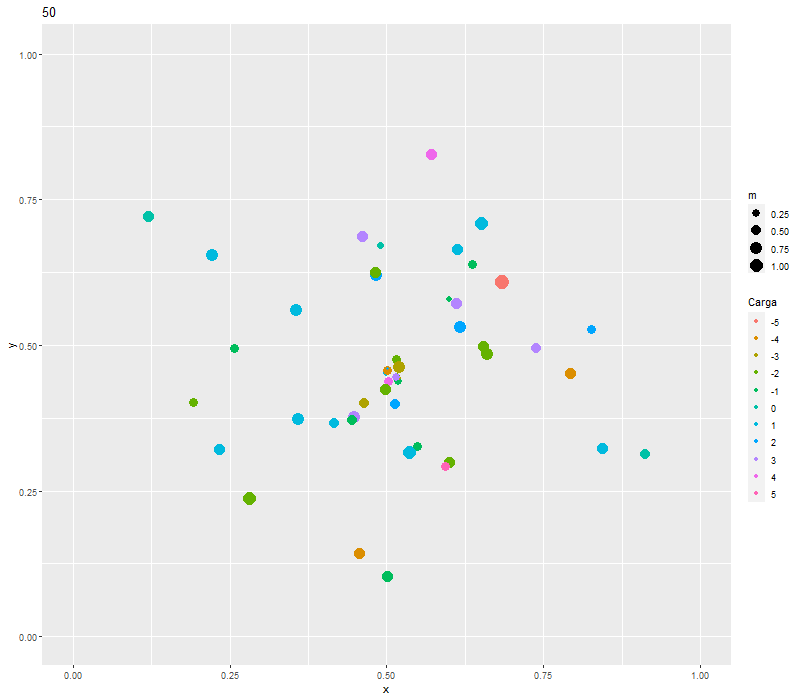
\includegraphics[width=\linewidth]{grafica10.png}
\caption{Paso 50.}
\label{f}
\end{subfigure}
\label{fig1}
\end{figure}


\section{Conclusiones}
De la práctica podemos concluir que a menor masa se tiene una mayor velocidad y esto se debe a que la velocidad resultante es fuertemente dependiente de las diversas masas que hay en el sistema lo cual es cierto para masas muy pequeñas. Cuando se tenían masas iguales no se observaron cambios entre las velocidades de las partículas ya que solo dependían de las cargas. De igual forma las de mayor masa presentan una menor velocidad y por eso no se observan grandes diferencias entre la mayoría de las partículas. De las pruebas no se obtuvieron datos con distribución normal y se rechazaban las hipótesis nulas donde no todas las medianas son iguales. 

\bibliography{referencias}
\bibliographystyle{plainnat}
\end{document}
